\section{Unstructured Data}

Unstructured data refers to information that does not follow a predefined schema or tabular format, making it inherently more complex to process and analyze than structured (typically stored in SQL databases) or semi-structured (typically managed by NoSQL databases) data. Examples include text documents, images, audio and video files, sensor logs, scientific data, and code, which vary widely in format, size, and origin and often require specialized techniques to extract meaningful insights.

\subsection{Embeddings}

Embeddings are numerical representations of data mapped into a continuous vector space (Figure~\ref{fig:data-1-a}), where semantically similar objects are placed close together (Figure~\ref{fig:data-1-b}). They bridge the gap between discrete, symbolic data and differentiable machine learning models, representing complex objects as fixed-length vectors. High-quality embeddings capture relevant features of the original data, supporting tasks such as classification, clustering, and similarity search \cite{Grohe-2020}.

\subsection{Distance Metrics}

Choosing an appropriate distance metric (Table~\ref{tab:distance-metrics}) ensures that embeddings accurately reflect the semantic similarity of the original unstructured data.

\begin{figure}[h]
    \centering
    \begin{subfigure}[t]{0.48\textwidth}
        \centering
        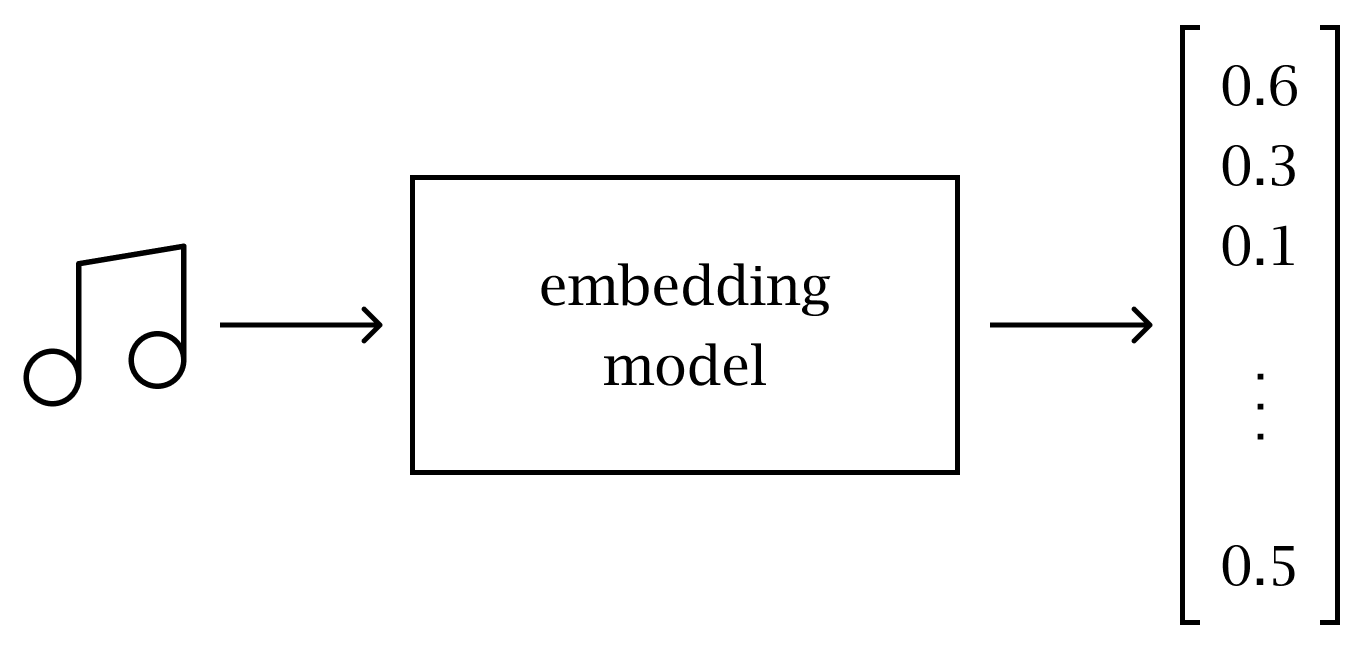
\includegraphics[width=\textwidth]{chapters/theory/data/figures/embedding.png}
        \caption{Unstructured data processed through a model to generate embeddings.}
        \label{fig:data-1-a}
    \end{subfigure}
    \hfill
    \begin{subfigure}[t]{0.48\textwidth}
        \centering
        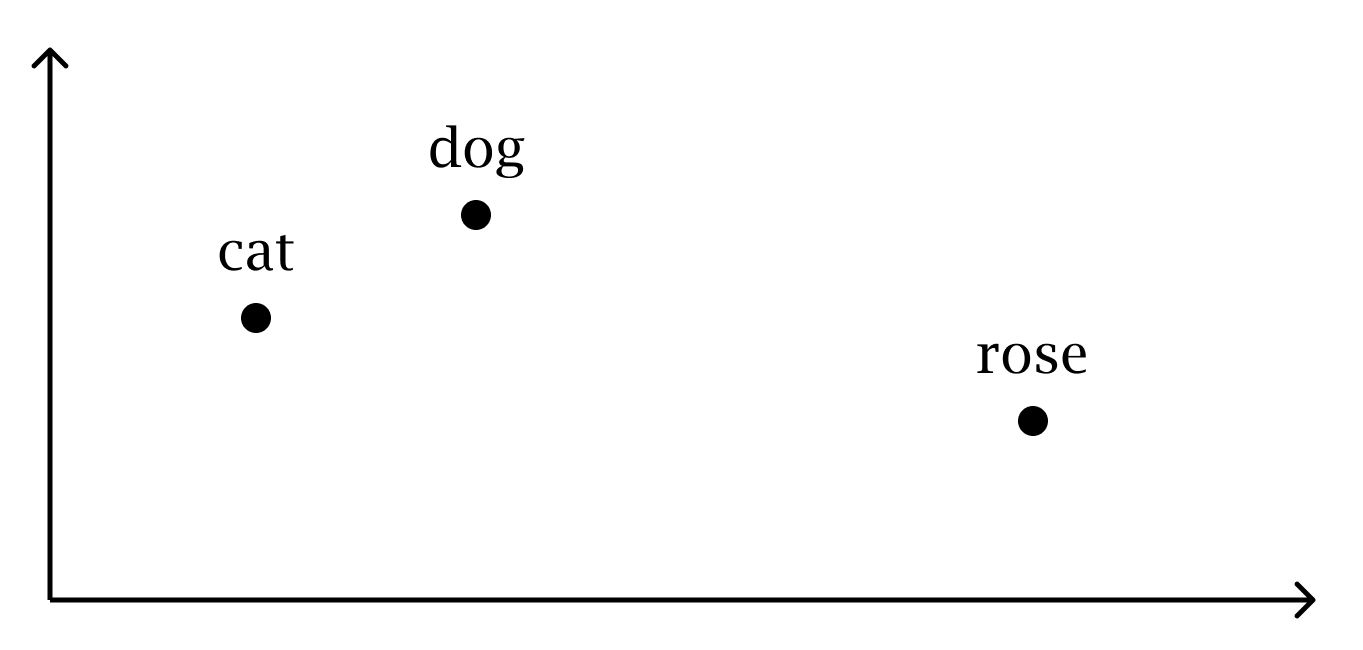
\includegraphics[width=\textwidth]{chapters/theory/data/figures/similarity.png}
        \caption{Semantically similar objects appear close together, while dissimilar ones are farther apart.}
        \label{fig:data-1-b}
    \end{subfigure}
    \caption{Illustration of the embedding process (a) and semantic similarity (b).}
    \label{fig:data-1}
\end{figure}

\begin{table}[h]
    \centering
    \renewcommand{\arraystretch}{2.3}
    \caption{Common similarity measures in vector databases.}
    \label{tab:distance-metrics}
    \begin{tabular}{|m{5cm}|m{8cm}|}
        \hline
        \textbf{Metric} & \textbf{Formula} \\ \hline
        $l_p$ (Minkowski) 
            & $\|x-y\|_p = \left(\sum_{i=1}^d |x_i-y_i|^p\right)^{1/p}$ \\ \hline
        $l_1$ (Manhattan) 
            & $\|x-y\|_1 = \sum_{i=1}^d |x_i-y_i|$ \\ \hline
        $l_2$ (Euclidean) 
            & $\|x-y\|_2 = \sqrt{\sum_{i=1}^d (x_i-y_i)^2}$ \\ \hline
        $l_\infty$ (Chebyshev) 
            & $\|x-y\|_\infty = \max_i |x_i-y_i|$ \\ \hline
        Cosine distance 
            & $d_{cos}(x,y) = 1 - (x \cdot y) / (\|x\|_2 \cdot \|y\|_2)
$ \\ \hline
        Dot (inner) product 
            & $s_{dot}(x,y) = \sum_{i=1}^d x_i \cdot y_i$ \\ \hline
        Hamming distance 
            & $d_{H}(x,y) = \sum_{i=1}^d 1(x_i \neq y_i)$ \\ \hline
    \end{tabular}
\end{table}